En este capítulo se abarcan los términos y tecnologías que serán utilizadas a lo largo del desarrollo del Trabajo Terminal, a fin de brindar un contexto más amplio para facilitar la comprensión del lector.
%--------------------------------------------------
\section{Aprendizaje máquina}
El aprendizaje máquina es un subcampo de Inteligencia Artificial (Artificial Intelligence, por sus siglas en inglés AI) que proporciona a los sistemas la capacidad de aprender y mejorar automáticamente a partir de la experiencia (registros almacenados en un repositorio de datos, fotos, música) sin estar explícitamente programados para resolver una tarea concreta. Se dice que el aprendizaje máquina hace uso de algoritmos genéricos sobre datos específicos y de esta manera se logra abordar problemas concretos.   
\\ \par 
Después de una breve introducción pasamos a una definición formal del aprendizaje máquina brindada por Tom M. Mitchell en 1997  ``Se dice que un programa de computadora aprende de la experiencia E con respecto a alguna clase de tareas T y la medida de rendimiento P si su desempeño en tareas en T, medido por P, mejora con la experiencia E'' \cite{mitchell}.
\\ \par
Una vez proporcionada una explicación formal del aprendizaje máquina hecha por uno de los contribuyentes más importantes en el campo, es necesario dar nombres y símbolos a los componentes principales de el problema de aprendizaje. Está la entrada x (características de los datos de entrada que se usan para tomar una decisión), la función objetivo desconocida $f: X \mapsto Y$ (fórmula ideal para descripción y/o predicción del problema a resolver), donde X es el espacio de entrada (conjunto de todas las posibles entradas x), e Y es el espacio de salida (conjunto de todas las salidas posibles). Hay un conjunto de datos D de ejemplos de entrada-salida (Datos de entrenamiento) $(x_1, y_1),(x_2,y_2), ... , (x_n, Y_n)$, donde $y_n = f(x_n)$ para $n = 1, ... , N$. Estos ejemplos a menudo se denominan puntos de datos \cite{Mostafa}. 
\\ \par
Otro componente de suma importancia es el algoritmo de aprendizaje $A$ que hace uso del conjunto de datos D para elegir una fórmula $g: X \mapsto Y$ que se aproxima a $f$. El algoritmo elige $g$ de un conjunto de fórmulas candidatas que llamamos conjunto de hipótesis H. 
Por ejemplo, H podría ser el conjunto de todas las fórmulas lineales a partir de las cuales el algoritmo elegiría el mejor ajuste lineal para los datos; La decisión será buena solo en la medida en que g se aproxime f. Para lograrlo, el algoritmo elige $g$ que mejor se adapte a $f$ en los datos de ejemplo provistos, con la esperanza de que el algoritmo generalice correctamente \cite{Mostafa}.
\\ \par
En la figura \ref{image:componentesmachine} podemos ver la manera en la que  los componentes de un problema de aprendizaje básico trabajan en conjunto.

\FloatBarrier
\begin{figure}[htbp!]
		\centering
			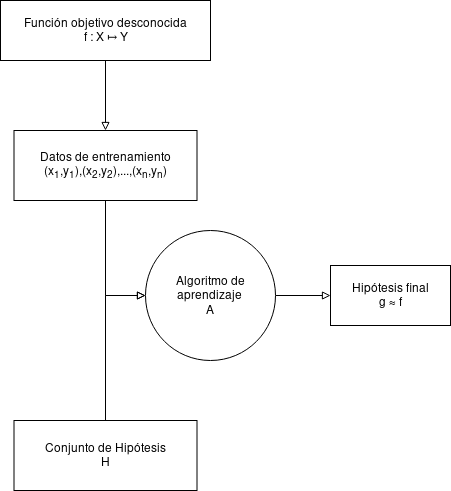
\includegraphics[width=.45 \textwidth]{imagenes/elementosAprendizaje}
		\caption{Diagrama de componentes básicos del problema de aprendizaje \cite{Mostafa}.}
		\label{image:componentesmachine}
\end{figure}


\FloatBarrier


\subsection{Antecedentes de la Inteligencia Artificial}
Al pertenecer el aprendizaje máquina al campo de la inteligencia artificial es pertinente mencionar los antecedentes que dieron paso a esta disciplina que ha estado perdiendo y recuperando importancia desde el primer momento en que fue mencionada.  \\
\subsubsection{Nacimiento [1952-1956]}
1950 - Alan Turing crea la ``Prueba de Turing'' para determinar si una máquina es realmente inteligente o no. Para pasar la prueba, la máquina debe ser capaz de hacer creer a un ser humano que se trata de otro ser humano en lugar de una computadora \cite{V.Gonzalez}.
\\ \par
1952 - Arthur Samuel escribe el primer programa de computadora capaz de aprender. El software era un programa que podía jugar a las damas y mejorar con cada juego que jugaba \cite{V.Gonzalez}.
\\ \par
1956 - Martin Minsky y John McCarthy, con la ayuda de Claude Shannon y Nathan Rochester, tuvieron una conferencia en Dartmouth en 1956, que se considera donde nació el campo de la Inteligencia Artificial. Minsky convenció a los asistentes a adoptar el término ``Inteligencia Artificial'' como el nombre del nuevo campo \cite{V.Gonzalez}.
\\ \par
1958 - Frank Rosenblatt diseña el Perceptron, la primera red neuronal artificial \cite{V.Gonzalez}.
\\ \par
\subsubsection{Primer invierno de la Inteligencia Artificial [1974-1980] }


En la segunda mitad de la década de 1970, el campo sufrió su primer ``invierno''. Varias agencias que habían estado financiando la investigación en AI cortaron fondos después de años de altas expectativas y pocos avances reales \cite{V.Gonzalez}.
\\ \par
1979 - Los estudiantes de la Universidad de Stanford inventan el ``Stanford Cart'', un robot móvil capaz de moverse de forma autónoma por una habitación evitando obstáculos \cite{V.Gonzalez}.
\\ \par
1967 - Se escribe el algoritmo ``Vecino más cercano''. Este hito se considera el nacimiento del campo del reconocimiento de patrones en las computadoras \cite{V.Gonzalez}. 
\\ \par

\subsubsection{La explosión de los 80's [1980-1987]}

Los años 80 se conocen como el nacimiento de sistemas expertos, basados en reglas. Estos fueron rápidamente adoptados por el sector corporativo, generando un nuevo interés en Machine Learning \cite{V.Gonzalez}.
\\ \par
1981 - Gerald Dejong introduce el concepto de ``Aprendizaje basado en la explicación'' (Explanation-Based Learning, por sus siglas en inglés EBL), en el que una computadora analiza los datos de capacitación y crea reglas generales que permiten descartar los datos menos importantes \cite{V.Gonzalez}.
\\ \par
1985 - Terry Sejnowski inventa NetTalk, que aprende a pronunciar palabras de la misma manera que un niño aprendería a hacer \cite{V.Gonzalez}.
\\ \par
\subsubsection{Segundo Invierno de la Inteligencia Artificial [1987-1993]}

A finales de la década de 1980 y principios de la década de 1990, AI experimentó un segundo ``invierno''. Esta vez, sus efectos duraron varios años y la reputación del campo no se recuperó por completo hasta principios de la década de 2000 \cite{V.Gonzalez}.
\\ \par
Década de 1990: el trabajo en Machine Learning se mueve de un enfoque basado en el conocimiento a uno basado en datos. Los científicos comienzan a crear programas que analizan grandes cantidades de datos y extraen conclusiones de los resultados \cite{V.Gonzalez}.
\\ \par
1997 - La computadora Deep Blue, IBM (International Business Machines), vence al campeón mundial de ajedrez Gary Kaspárov \cite{V.Gonzalez}. 
\\ \par
\subsubsection{Explosión y adopción comercial [2006-Actual]}

El crecimiento en el potencial de cálculo junto con la gran abundancia de datos disponibles han relanzado el campo del aprendizaje automático. Muchas empresas están moviendo sus empresas hacia los datos e incorporando Machine Learning en sus procesos, productos y servicios con el fin de obtener una ventaja sobre su competencia \cite{V.Gonzalez}.
\\ \par
2006 - Geoffrey Hinton acuñó la frase ``Aprendizaje Profundo'' (Deep Learning, por sus siglas en inglés DL) para explicar las nuevas arquitecturas de redes neuronales profundas capaces de aprender modelos mucho mejores \cite{V.Gonzalez}.
\\ \par
2011 - La computadora Watson de IBM supera a sus competidores humanos en Jeopardy, un juego que consiste en responder preguntas en lenguaje natural \cite{V.Gonzalez}.
\\ \par
2012 - Jeff Dean, en Google, con la asistencia de Andrew Ng (Universidad de Stanford), lidera el proyecto GoogleBrain, que desarrolló una red neuronal profunda utilizando toda la capacidad de la infraestructura de Google para detectar patrones en videos e imágenes \cite{V.Gonzalez}.
\\ \par
2012 - Geoffrey Hinton lidera el equipo ganador en el concurso de Visión por computadora en Imagenet utilizando una Red Neuronal Profunda (Deep Neuronal Network, por sus siglas en inglés DNN). El equipo ganó por un amplio margen, dando lugar a la explosión actual de Machine Learning basada en DNN \cite{V.Gonzalez}.
\\ \par
2012 - El laboratorio de investigación Google X utiliza GoogleBrain para analizar de forma autónoma videos de YouTube y detectar aquellos que contienen gatos \cite{V.Gonzalez}.
\\ \par
2014 - Facebook desarrolla DeepFace, un algoritmo basado en DNN capaces de reconocer a las personas con la misma precisión que un ser humano \cite{V.Gonzalez}.
\\ \par
2014 - Google compra DeepMind, una startup británica de aprendizaje profundo que recientemente ha demostrado las capacidades DNN con un algoritmo capaz de jugar juegos Atari simplemente viendo los píxeles en la pantalla, de la misma manera que lo haría una persona. El algoritmo, después de horas de entrenamiento, era capaz de vencer a expertos humanos en los juegos \cite{V.Gonzalez}.
\\ \par
2015 - Amazon lanza su propia plataforma de Machine Learning \cite{V.Gonzalez}.
\\ \par
2015: Microsoft crea el ``Kit de herramientas para el aprendizaje de máquinas distribuidas'', que permite la distribución eficiente de problemas de aprendizaje automático en varias computadoras \cite{V.Gonzalez}.
\\ \par
2015 - Elon Musk y Sam Altman, entre otros, fundan la organización sin fines de lucro OoenAI, dándole mil millones de dólares con el objetivo de garantizar que la inteligencia artificial tenga un impacto positivo en la humanidad \cite{V.Gonzalez}.
\\ \par
2016 - Google DeepMind vence al jugador profesional de Go, Lee Sedol, de cinco juegos a uno en lo que se considera uno de los juegos de mesa más complejos. Los jugadores de Expert Go confirmaron que el algoritmo era capaz de realizar movimientos ``creativos'' que nunca habían visto antes \cite{V.Gonzalez}.
\\ \par
Hoy, estamos experimentando una tercera explosión en inteligencia artificial. Aunque hay escépticos que dicen que no podemos descartar la posibilidad de un tercer invierno, esta vez los avances en el sector se están aplicando a las empresas hasta el punto de crear mercados completamente nuevos y producir cambios significativos en las estrategias de las grandes y pequeñas empresas \cite{V.Gonzalez}.
\\ \par
La amplia disponibilidad de datos parece ser el combustible detrás de estos motores de algoritmo que, a su vez, están sobrepasando las limitaciones de cálculo que existían antes de la computación distribuida. Todo esto parece indicar que deberíamos seguir teniendo acceso a más y más datos que alimentarán nuestros algoritmos; la comunidad científica no parece quedarse sin ideas para seguir avanzando en el campo. 2017 y los años siguientes prometen ser realmente frenéticos \cite{V.Gonzalez}.
\\ \par 
\subsection{Tipos de aprendizaje}
La premisa básica de aprender de datos haciendo uso de un conjunto de observaciones para predecir el resultado de un proceso o descubrir un patrón oculto a simple vista es una premisa muy amplia y difícil de encajar en un marco único. Como resultado, han surgido diferentes paradigmas de aprendizaje para tratar las múltiples situaciones que se pueden presentar. En esta sección, presentamos algunos de estos paradigmas \cite{Mostafa}.
\\
% - - - - - - - - - - - - - - - - - - - - - - - - -
\subsubsection{Aprendizaje supervisado}
La mayoría del aprendizaje automático en la práctica utiliza el aprendizaje supervisado. El aprendizaje supervisado se aplica cuando se tienen variables de entrada (X) y una variable de salida (Y) ya conocida, dicho paradigma utiliza un algoritmo para aprender la función de mapeo desde la entrada hasta la salida.
\FloatBarrier

\begin{equ}[!ht]
  \begin{equation}
   Y = f(X)
  \end{equation}
 \caption{Función de mapeo \cite{Mostafa}.}
 \label{equation:mapeo}
\end{equ}
\FloatBarrier

El objetivo es aproximar la función de mapeo tan bien que cuando tenga datos de entrada nuevos (X) pueda predecir las variables de salida (Y) para esos datos (Ecuación \ref{equation:mapeo}).\\

Se denomina aprendizaje supervisado porque el proceso de aprendizaje de un algoritmo a partir del conjunto de datos de capacitación puede considerarse como un maestro que supervisa el proceso de aprendizaje. Conocemos las respuestas correctas, el algoritmo realiza predicciones de forma iterativa sobre los datos de entrenamiento y es corregido por el profesor. El aprendizaje se detiene cuando el algoritmo alcanza un nivel aceptable de rendimiento \cite{Mostafa}.


\subsection{Aprendizaje no supervisado}
El aprendizaje no supervisado se aplica en casos cuando solo tienes datos de entrada (X) y no hay variables de salida correspondientes. El objetivo del aprendizaje no supervisado es modelar la estructura o distribución subyacente en los datos para aprender más sobre los datos. Estos se llaman aprendizaje no supervisado porque a diferencia del paradigma anterior, no hay respuestas correctas y no hay profesor. Los algoritmos se dejan a sus propios dispositivos para descubrir y presentar la estructura interesante en los datos. Los problemas de aprendizaje sin supervisión se pueden agrupar en problemas de agrupamiento y asociación \cite{Mostafa}. \\


\begin{itemize}
\item Agrupamiento: Un problema de agrupamiento, como lo dice su nombre, consiste en encontrar distintos grupos que contengan características en común dentro de grandes cantidades de datos \cite{Mostafa}.

\item Asociación: Un problema de asociación se basa en encontrar comportamientos que se describen mediante reglas como: si pasa X entonces tiende a pasar Y. Estas reglas (llamadas formalmente reglas de asociación) se pueden ver muy reflejadas en las compras en un supermercado; los clientes que suelen comprar el producto X también compran el producto Y \cite{Mostafa}. 
\end{itemize}

\subsubsection{Algoritmo de agrupamiento K-means}

K-means (MacQueen, 1967) es uno de los algoritmos de aprendizaje no supervisado más simples que resuelven el conocido problema de agrupamiento. El procedimiento sigue una forma simple y fácil de clasificar un conjunto de datos dado a través de un cierto número de agrupaciones (suponga k agrupaciones) fijadas a priori. La idea principal es definir k centroides, uno para cada grupo. Estos centroides deben colocarse de forma astuta debido a que la ubicación diferente causa un resultado diferente. Entonces, la mejor opción es colocarlos lo más lejos posible unos de otros. El siguiente paso es tomar cada punto que pertenezca a un conjunto de datos determinado y asociarlo al centroide más cercano. Cuando no hay ningún punto pendiente, se completa el primer paso y se realiza una agrupación temprana. En este punto, necesitamos volver a calcular k nuevos centroides como baricentros de los grupos resultantes del paso anterior. Una vez que tengamos estos k nuevos centroides, se debe realizar un nuevo enlace entre los mismos puntos de conjunto de datos y el nuevo centroide más cercano. Se ha generado un bucle. Como resultado de este bucle, podemos observar que los k centroides cambian su ubicación paso a paso hasta que no se realicen más cambios. En otras palabras, los centroides ya no se mueven.
Finalmente, este algoritmo apunta a minimizar una función objetivo, en este caso una función de error al cuadrado. La funcion de error es la siguiente: \cite{kmeans}
\FloatBarrier

\begin{equ}[!ht]
  \begin{equation}
         J = \sum_{j = 1}^{k} \sum_{i=0}^{N} {|| {x_i}^{(j)} - c_j ||}^2
  \end{equation}
 \caption{Función de error K-means \cite{kmeans}.}
  \label{equation:jmeans}
\end{equ}
\FloatBarrier

Donde \ref{equation:jmeans} es una medida de distancia elegida entre un punto $ {x_i}^{(j)}$ de datos y el centro del clúster $ c_j $, En otras palabras, es un indicador de la distancia de los n puntos de datos desde sus respectivos centros de clúster.
\\El algoritmo para el agrupamiento K-means es el siguiente (La cuál fue obtenida de   \cite{kmeans}):
\begin{enumerate}
\item Coloque K puntos en el espacio representado por los objetos que se agrupan. Estos puntos representan los centroides del grupo inicial.
\item Asigne cada objeto al grupo que tenga el centroide más cercano.
\item Cuando todos los objetos hayan sido asignados, vuelva a calcular las posiciones de los K centroides.
\item Repita los pasos 2 y 3 hasta que los centroides ya no se muevan. Esto produce una separación de los objetos en grupos a partir de los cuales se puede calcular la métrica a minimizar.
\end{enumerate}

Finalmente, una representación gráfica de el resultado de ejecutar K-means con $K = 3$ sobre un conjunto de datos se puede visualizar en la figura \ref{image:kmeans}

\FloatBarrier
\begin{figure}[htbp!]
		\centering
			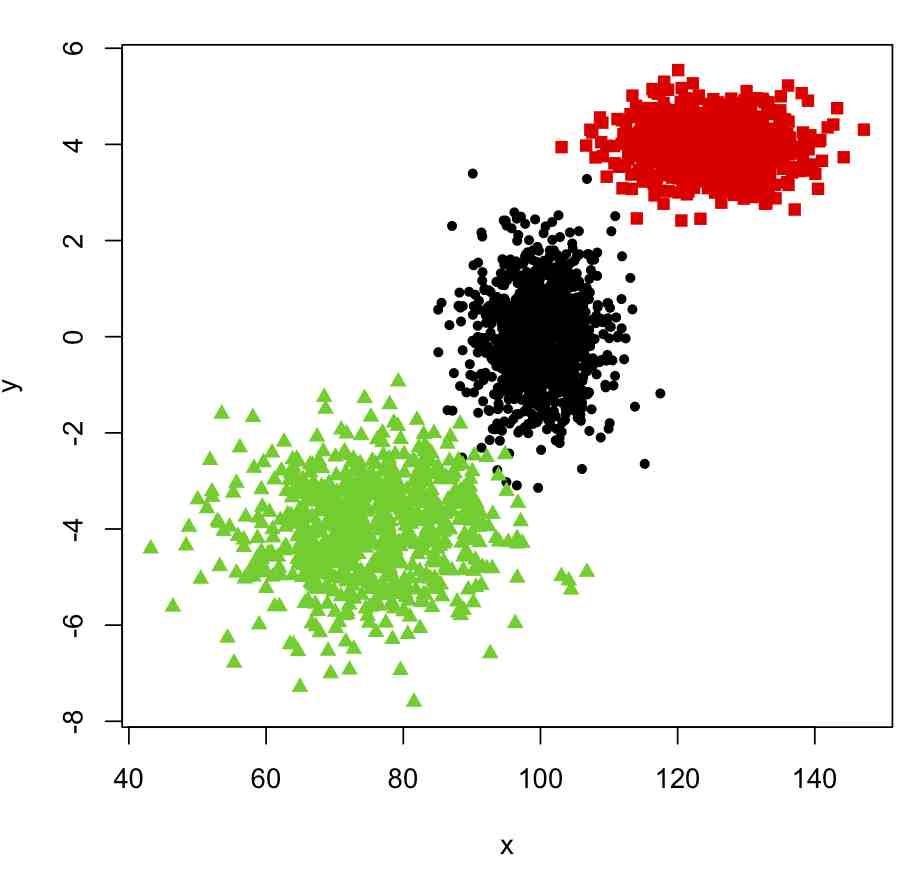
\includegraphics[width=.45 \textwidth]{imagenes/kmeans}
		\caption{Ejemplo de agrupamiento con K-means \cite{kmeansimage}. }
		\label{image:kmeans}
\end{figure}


\FloatBarrier


% - - - - - - - - - - - - - - - - - - - - - - - - 

\subsection{Algoritmos de Aprendizaje supervisado}
En esta sección se explicarán algunos algoritmos pertenecientes al paradigma de Aprendizaje Supervisado pero antes de realizar la explicación es necesario familiarizarse con algunas técnicas y términos. \\

\subsubsection{Hiperplano}
Un hiperplano es un subespacio lineal de dimesión $n-1$ que separa en un espacio de dimensión n en dos mitades. Todo hiperplano en $\mathbb{R}^n $ se describe mediante la ecuación número \ref{equation:hiperplano}.
\FloatBarrier

\begin{equ}[!ht]
  \begin{equation}
         \sum_{i = 1}^{n} a_i x_i = \Theta  
  \end{equation}
 \caption{Definición matemática de un hiperplano  \cite{Tema 5 Aprendizaje automatico}.}
  \label{equation:hiperplano}
\end{equ}
\FloatBarrier

\subsubsection{Separabilidad lineal}
La separabilidad lineal se define en la ecuación \ref{equation:separabilidad-lineal} de la siguiente manera: Dos conjuntos $M_1 \in \mathbb{R}^n $ y $M_2 \in \mathbb{R}^n $ son linealmente separables si existen números $a_1, a_2, ... , a_n, \Theta$ tales que 
\FloatBarrier

\begin{equ}[!ht]
   \begin{equation}
	\forall x \in M_1  \sum_{i = 1}^{n} a_i x_i > \Theta \textbf{ y } \forall x \in M_2  \sum_{i = 1}^{n} a_i x_i \leq \Theta
  \end{equation}
 \caption{Definición matemática de separabilidad lineal \cite{Tema 5 Aprendizaje automatico}.}
 \label{equation:separabilidad-lineal}
\end{equ}
\FloatBarrier

Donde al valor de $\Theta$ se le denomina umbral.

\subsubsection{Red neuronal artificial}

La definición más simple de una red neuronal, más propiamente llamada Red Neuronal Artificial (Artificial Neuronal Network, por sus siglas en inglés ANN), la proporciona el inventor de uno de los primeros neurocomputadores, el Dr. Robert Hecht-Nielsen. Él define una red neuronal como: ``\textit{... un sistema informático compuesto por una serie de elementos de procesamiento simples, altamente interconectados, que procesan la información por su respuesta de estado dinámico a las entradas externas.}'' en ``Neural Network Primer: Part I'' por Maureen Caudill, AI Expert, febrero de 1989. Las RNA son dispositivos de procesamiento (algoritmos o hardware real) que se modelan de forma flexible basadas en la estructura neuronal de la corteza cerebral, pero a escalas mucho más pequeñas. Una ANN grande puede tener cientos o miles de unidades de procesador, mientras que un cerebro tiene miles de millones de neuronas con un aumento correspondiente en la magnitud de su interacción global y comportamiento emergente \cite{A Basic Introduction To Neural Networks}. \\

\paragraph{Elementos de una red neuronal} ~\\
 
Las redes neurales se organizan típicamente en capas. Las capas están formadas por una serie de 'nodos' interconectados que contienen una 'función de activación'. Los patrones se presentan en la red a través de la capa de entrada, que se comunica con una o más capas ocultas donde el procesamiento real se realiza a través de un sistema de 'conexiones' ponderadas. Las capas ocultas se vinculan a una capa de salida donde la respuesta se muestra como se muestra como en la figura \ref{image:redneuronaldiagrama} \cite{A Basic Introduction To Neural Networks}.

\FloatBarrier
\begin{figure}[htbp!]
		\centering
			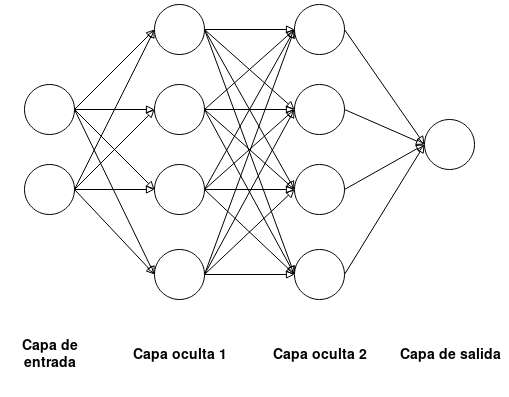
\includegraphics[width=.45 \textwidth]{imagenes/red_neuronal}
		\caption{Diagrama de una red neuronal.}
		\label{image:redneuronaldiagrama}
\end{figure}


\FloatBarrier


\paragraph{Función de activación} ~\\

Consideremos la neurona que se muestra en la ecuación \ref{equation:definicionneurona}. 

\FloatBarrier
\begin{equ}[!ht]
  \begin{equation}
	Y = \sum_{i = 0}^{n}({\theta}_i x_i)    
 \end{equation}
 \caption{Definición matemática de una neurona. \cite{Andrew} }
 \label{equation:definicionneurona}
\end{equ}
\FloatBarrier

El valor de Y puede ser cualquier valor desde $-\infty$ a $+\infty$. La neurona realmente no conoce los límites del valor. Entonces, ¿cómo decidimos si la neurona debe ser activada o no? para solucionar este problema decidimos agregar funciones de activación que verifican el valor Y producido por una neurona y toman la decisión de si las conexiones externas deberían considerar esta neurona como activada o no \cite{NeuralNetworks}. Algunas de las funciones de activación más utilizadas son las siguientes: \\
\begin{itemize}
\item Función Escalón unitario,
\item Función Sigmoide,
\item Función Tangente Hiperbólica,
\item Función Rectificadora.
\end{itemize}

\subsubsection{Perceptrón}
Es un algoritmo de clasificación muy simple que equivale a una red neuronal de dos capas (capa de entrada y capa de salida) que usualmente va de la mano de la función de activación escalón unitario (Threshold) o la función signo (Sign). Dentro de esta red neuronal cada nodo representa una neurona artificial y cada enlace  simula la sinapsis que ocurre en las neuronas biológicas.
\\ \par
Los elementos de un perceptrón se definen como $\theta = ({\theta}_1, {\theta}_2, ... , {\theta}_n) \in \mathbb{R}^n$ que denota el vector de pesos y $X \in \mathbb{R}^n$ el vector de entradas. Un perceptrón se define como la función de mapeo $P : X \in \mathbb{R}^n \mapsto \left\{-1,+1\right\}$ que se puede escribir como se muestra en la ecuación \ref{equation:perceptron}. 

\FloatBarrier

\begin{equ}[!ht]
  \begin{equation}
	P(x)=
      \left\{ \begin{array}{ll}
            +1, & Si \sum_{i = 1}^{n} {\theta}_i x_i > \Theta  \\
           -1 & \textit{En otro caso}
        \end{array} \right.     
  \end{equation}
 \caption{Definición matemática del Perceptrón. \cite{Tema 5 Aprendizaje automatico}}
 \label{equation:perceptron}
\end{equ}
\FloatBarrier


Observe que las variables $x_i$ corresponden a cada elemento del vector de entradas X que serán tomadas en cuenta durante la clasificación. Como se puede observar en la fórmula $\sum_{i = 1}^{n} {\theta}_i x_i > \Theta $, todos los puntos por encima del hiperplano $\sum_{i = 1}^{n} {\theta}_i x_i = \Theta $ se clasifican como positivos y los restantes como negativos. El algoritmo de aprendizaje más básico del perceptrón se define de la manera siguiente: \\

\tab \tab \tab \tab \tab Perceptron($M_+, M_-$)\\
\tab \tab \tab \tab \tab w = vector aleatorio de números reales \\
\tab \tab \tab \tab \tab Repetir hasta que $x \in M_+ \cup M_-$ esté clasificado correctamente \\
\tab \tab \tab \tab \tab \tab $\forall x \in M_+$ \\
\tab \tab \tab \tab \tab \tab \tab si $xw \leq \Theta $ entonces ${\theta} += x$\\
\tab \tab \tab \tab \tab \tab $\forall x \in M_-$ \\
\tab \tab \tab \tab \tab \tab \tab si $xw > \Theta $ entonces ${\theta} -= x$ \cite{Andrew}\\

Donde $M_+$ y $M_-$ representan a los datos de entrenamiento positivos y negativos respectivamente. El perceptrón deberá asignar la salida de +1 a todo $x \in M_+$ y -1 a todo $x \in M_-$. Si el perceptrón clasifica erróneamente se hace el ajuste del vector de pesos para modificar éste en la dirección correcta. En la figura \ref{image:perceptonclasificacion} se puede apreciar el resultado final de un proceso de clasificación hecho con un perceptrón.

\FloatBarrier
\begin{figure}[htbp!]
		\centering
			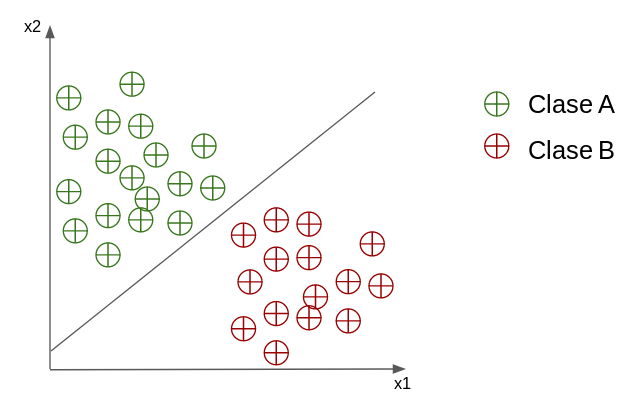
\includegraphics[width=.5 \textwidth]{imagenes/perceptron}
		\caption{Función de clasificación lineal ${\theta}_1 x_1 + {\theta}_2 x_2 = -b$.}
		\label{image:perceptonclasificacion}
\end{figure}
\FloatBarrier


\subsubsection{Sistemas de recomendación}

Un sistema de recomendación se define como una estrategia de toma de decisiones para los usuarios en entornos de información complejos. También ha sido definido desde la perspectiva del comercio electrónico como una herramienta que ayuda a los usuarios a buscar a través de registros de conocimiento que están relacionados con los intereses y preferencias de éstos mismos. Por otro lado, se definió como un medio para ayudar y aumentar el proceso social de usar recomendaciones de otros para tomar decisiones cuando no hay suficiente conocimiento personal o experiencia de las alternativas. Los sistemas de recomendación manejan el problema de la sobrecarga de información que los usuarios normalmente encuentran al proporcionarles recomendaciones de servicio y contenido personalizado y exclusivo. Recientemente, se han desarrollado varios enfoques para construir sistemas de recomendación, que pueden utilizar el filtrado colaborativo, el filtrado basado en contenido o el filtrado híbrido \cite{Isinkaye}. Cada una de estas técnicas serán explicadas a continuación.\\

\paragraph{Enfoque basado en contenido} ~\\

La técnica basada en contenido es un algoritmo que se enfatiza en el análisis de los atributos de los artículos para generar predicciones. Cuando se recomiendan documentos como sitios Web, publicaciones y noticias, la técnica de filtrado basada en el contenido es la más exitosa. En la técnica de filtrado basada en contenido, la recomendación se basa en los perfiles de usuario que utilizan características extraídas del contenido de los artículos que el usuario ha evaluado en el pasado. Los artículos que están relacionados principalmente con los artículos calificados positivamente se recomiendan para el usuario. El Enfoque Basado en Contenido (Content Based Focus, por sus siglas en inglés CBF) utiliza diferentes tipos de modelos para encontrar similitud entre los documentos a fin de generar recomendaciones significativas. Podría utilizar Modelo de espacio vectorial o modelos probabilísticos como Clasificador bayesiano ingenuo, árboles de decisión o redes neuronales artificiales para modelar la relación entre las diferentes características dentro de un producto/documento. Estas técnicas hacen recomendaciones aprendiendo el modelo subyacente con análisis estadístico o técnicas de aprendizaje automático. La técnica de filtrado basada en contenido no necesita el perfil de otros usuarios, ya que no influyen en la recomendación. Además, si el perfil del usuario cambia, la técnica CBF todavía tiene el potencial de ajustar sus recomendaciones en un período de tiempo muy corto. La principal desventaja de esta técnica es la necesidad de tener un conocimiento profundo y una descripción de las características de los artículos en el perfil \cite{Isinkaye}. 

\paragraph{Enfoque basado en filtrado colaborativo} ~\\

El filtrado colaborativo es una técnica de predicción para contenido que no puede describirse de manera fácil y adecuada mediante metadatos, como películas o música. La técnica de filtrado colaborativo funciona mediante la creación de una base de datos (matriz Usuario-Artículo) de las preferencias de los artículos por parte de los usuarios. A continuación, compara usuarios con intereses y preferencias relevantes calculando similitudes entre sus perfiles para hacer recomendaciones. Dichos usuarios crean un grupo llamado barrio. Un usuario recibe recomendaciones para aquellos artículos que no ha calificado anteriormente pero que ya fueron calificados positivamente por los usuarios de su vecindario. Las recomendaciones que produce FC pueden ser de predicción o recomendación. La predicción es un valor numérico, $R_{ij}$, que expresa la puntuación pronosticada del ítem j para el usuario i, mientras que la Recomendación es una lista de los N artículos principales que más le gustarán al usuario, como se muestra en la figura \ref{image:filtradocolaborativo}. La técnica de filtrado colaborativo puede ser dividido en dos categorías: basado en la memoria y basado en modelos \cite{Isinkaye}. 

\FloatBarrier
\begin{figure}[htbp!]
		\centering
			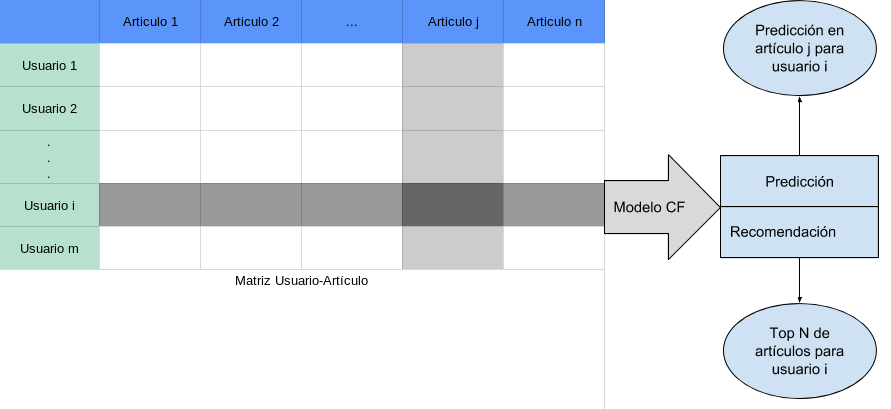
\includegraphics[width=.9 \textwidth]{imagenes/filtrado_colavorativo}
		\caption{Proceso de filtrado colaborativo \cite{Isinkaye}. }
		\label{image:filtradocolaborativo}
\end{figure}
\FloatBarrier

\paragraph{Filtrado colaborativo: Basado en memoria} ~\\

Los artículos que ya fueron calificados por el usuario antes desempeñan un papel relevante en la búsqueda de un vecino que comparta gustos con él. Una vez que se encuentra el vecino de un usuario, se pueden usar diferentes algoritmos para combinar las preferencias de los vecinos para generar recomendaciones. Debido a la efectividad de estas técnicas, han logrado un gran éxito en aplicaciones de la vida real. El FC basada en la memoria se puede lograr de dos maneras a través de técnicas basadas en el usuario y en artículo. La técnica de filtrado colaborativo basada en el usuario calcula la similitud entre usuarios al comparar sus calificaciones en el mismo artículo, y luego calcula la calificación pronosticada para un artículo por el usuario activo como un promedio ponderado de las calificaciones del artículo por usuarios similares al usuario activo. Las técnicas de filtrado basadas en artículos calculan predicciones utilizando la similitud entre los artículos y no la similitud entre los usuarios. Construye un modelo de similitudes de artículo recuperando todos los artículos calificados por un usuario activo de la matriz de Usuario-Artículo, determina qué tan similares son los artículos recuperados al artículo destino, luego selecciona los k artículos más similares y sus similitudes correspondientes. La predicción en este enfoque se realiza tomando un promedio ponderado de la calificación de usuarios activos en los artículos similares k. Se utilizan varios tipos de medidas de similitud para calcular la similitud entre el artículo / usuario. Las dos medidas de similitud más populares están basadas en correlación y en coseno. El coeficiente de correlación de Pearson se utilizada para medir el nivel en que dos variables aleatorias cuantitativas se relacionan linealmente entre sí. Este coeficiente se define como se muestra en la ecuación \ref{equation:coeficientepearson} \cite{Isinkaye}. 
\FloatBarrier
\begin{equ}[!ht]
  \begin{equation}
	s(a,u) = \frac{\sum_{i = 1}^{n}(r_{a,i} - \overline{r_a})(r_{u,i} - \overline{r_u}) }{\sqrt{\sum_{i = 1}^{n}(r_{a,i} - \overline{r_a})^2} \sqrt{\sum_{i = 1}^{n}(r_{u,i} - \overline{r_u})^2}}    
 \end{equation}
 \caption{Definición matemática de coeficiente de correlación de Pearson \cite{Isinkaye}.}
 \label{equation:coeficientepearson}
\end{equ}
\FloatBarrier

De la ecuación anterior, $s(a,u)$ denota la similitud entre dos usuarios a y u, $r_{a,i}$ es la calificación otorgada al artículo i por el usuario a, $r_a$ es la calificación promedio dada por el usuario a mientras que n es el número total de elementos en el espacio Usuario-Artículo. Además, la predicción para un artículo se realiza a partir de la combinación ponderada de las calificaciones de los vecinos seleccionados, que se calcula como la desviación ponderada de la media de los vecinos. La fórmula de predicción general es (ecuación \ref{equation:similitudcoseno}) \cite{Isinkaye}:

\FloatBarrier
\begin{equ}[!ht]
  \begin{equation}
	p(a,i) = \overline{r_a} + \frac{\sum_{i=1}^{n}(r_{u,i} - \overline{r_u}) \times s(a,u)}{\sum_{i=1}^{n}s(a,u)}  
 \end{equation}
 \caption{Definición matemática de fórmula de predicción \cite{Isinkaye}.}
 \label{equation:similitudcoseno}
\end{equ}
\FloatBarrier
La similitud del coseno es diferente de la medida basada en Pearson porque es un modelo vectorial-espacial que se basa en el álgebra lineal más que en el enfoque estadístico. Mide la similitud entre dos vectores n-dimensionales en función del ángulo que los separa. La medida basada en coseno se utiliza ampliamente en los campos de la recuperación de información y extracción de textos para comparar dos documentos de texto, en este caso, los documentos se representan como vectores de términos. La similitud entre dos artículos u y v se puede definir con la ecuación 2.8 \cite{Isinkaye}: 

\FloatBarrier
\begin{equ}[!ht]
  \begin{equation}
	s(\vec{u},\vec{v}) = \frac{\vec{u}\cdot\vec{v}}{\mid \vec{u} \mid * \mid \vec{v} \mid } = \frac{\sum_{i}(r_{u,i}r_{v,i})}{\sqrt{\sum_{i}r_{u,i}^2} \times \sqrt{\sum_{i}r_{v,i}^2}}
 \end{equation}
 \caption{Definición matemática de similitud del coseno \cite{Isinkaye}.}
\end{equ}
\FloatBarrier

La medida de similitud también se conoce como métrica de similitud, y son métodos utilizados para calcular los puntajes que expresan que tan similares son los usuarios o artículos. Estos puntajes se pueden usar como base para la generación de recomendaciones basadas en usuarios o en artículos. Dependiendo del contexto de uso, las métricas de similitud también pueden denominarse métricas de correlación o métricas de distancia \cite{Isinkaye}.


\paragraph{Filtrado colaborativo: Basado en modelos} ~\\

Esta técnica emplea las clasificaciones anteriores para aprender un modelo con el fin de mejorar el rendimiento de la técnica de filtrado colaborativo (Colaborative Filter, por sus siglas en inglés CF). El proceso de construcción del modelo se puede hacer usando técnicas de aprendizaje máquina o minería de datos. Estas técnicas pueden recomendar rápidamente un conjunto de elementos por el hecho de que usan un modelo precalculado y han demostrado producir resultados de recomendación que son similares a las técnicas de recomendación basadas en el vecindario. Entre los ejemplos de estas técnicas se incluyen la técnica de reducción de la dimensionalidad, como la descomposición del valor singular (Singular Value Descomposition, por sus siglas en inglés SVD), la técnica de finalización de la matriz, los métodos semánticos latentes y la regresión y agrupamiento. Las técnicas basadas en modelos analizan la matriz de elementos de usuario para identificar las relaciones entre los elementos; usan estas relaciones para comparar la lista de recomendaciones de N principales. Las técnicas basadas en modelos resuelven los problemas de dispersión asociados con los sistemas de recomendación \cite{Isinkaye}.
\\ \par
El uso de algoritmos de aprendizaje también ha cambiado la forma en que los sistemas de recomendación pasaron de qué consumir a cuándo consumir realmente un producto. Por lo tanto, es muy importante examinar otros algoritmos de aprendizaje utilizados en los sistemas de recomendación basados en modelos \cite{Isinkaye}:
\begin{itemize}
\item Reglas de asociación,
\item Agrupamiento,
\item Árboles de decisión,
\item Redes neuronales artificiales,
\item Análisis de enlaces,
\item Regresión,
\item Clasificadores Bayesianos.
\end{itemize}

\paragraph{Pros y contras del filtrado colaborativo} ~\\

El filtrado colaborativo tiene algunas ventajas importantes sobre CBF ya que puede funcionar en dominios donde no hay mucho contenido asociado con los elementos y donde el contenido es difícil de analizar para un sistema informático. Además, la técnica CF tiene la capacidad de proporcionar recomendaciones fortuitas, lo que significa que puede recomendar elementos que son relevantes para el usuario, incluso sin que el contenido esté en el perfil del usuario. A pesar del éxito de las técnicas de CF, su uso generalizado ha revelado algunos problemas potenciales, como los siguientes \cite{Isinkaye}.

\begin{itemize}
\item \textbf{Inicio frío}: Esto se refiere a una situación en la que un sistema de recomendaciones no cuenta con información adecuada sobre un usuario o un elemento para hacer predicciones relevantes. Este es uno de los principales problemas que reduce el rendimiento del sistema de recomendaciones. El perfil de dicho nuevo usuario o artículo estará vacío ya que no ha calificado ningún elemento; por lo tanto, su gusto no es conocido por el sistema \cite{Isinkaye}.

\item \textbf{Dispersión de datos}: Este es el problema que ocurre como resultado de la falta de información, es decir, cuando solo algunos de los artículos disponibles en una base de datos son calificados por los usuarios. Esto siempre conduce a una matriz de elementos de usuario dispersa, incapacidad para localizar vecinos exitosos y, finalmente, la generación de recomendaciones débiles. Además, la escasez de datos siempre conduce a problemas de cobertura, que es el porcentaje de elementos en el sistema que para el cual se pueden hacer recomendaciones \cite{Isinkaye}.

\item \textbf{Escalabilidad}: Este es otro problema asociado con los algoritmos de recomendación porque el cálculo normalmente crece linealmente con la cantidad de usuarios y elementos. Una técnica de recomendación que sea eficiente cuando el número de conjunto de datos es limitado puede no ser capaz de generar un número satisfactorio de recomendaciones cuando se aumenta el volumen del conjunto de datos. Por lo tanto, es crucial aplicar técnicas de recomendación que sean capaces de escalar de manera exitosa a medida que aumenta el número de conjuntos de datos en una base de datos. Los métodos utilizados para resolver problemas de escalabilidad y acelerar la generación de recomendaciones se basan en técnicas de reducción de dimensionalidad, como el método de descomposición de valores singulares (SVD), que tiene la capacidad de producir recomendaciones confiables y eficientes \cite{Isinkaye}. 

\end{itemize}
\paragraph{Filtrado híbrido} ~\\

La técnica de filtrado híbrido combina diferentes técnicas de recomendación para obtener una mejor optimización del sistema para evitar algunas limitaciones y problemas de los sistemas de recomendación puros. La idea detrás de las técnicas híbridas es que una combinación de algoritmos proporcionará recomendaciones más precisas y efectivas que un solo algoritmo, ya que las desventajas de un algoritmo pueden ser superadas por otro algoritmo. El uso de múltiples técnicas de recomendación puede suprimir las debilidades de una técnica individual en un modelo combinado. La combinación de enfoques se puede realizar de cualquiera de las siguientes maneras: implementación separada de algoritmos y combinación del resultado, utilizando algunos filtros basados en contenido en enfoque colaborativo, utilizando algunos filtros colaborativos en enfoque basado en contenido, creando un sistema de recomendación unificado que brinde juntos ambos enfoques \cite{Isinkaye}.


%--------------------------------------------------
\newpage
\section{IoE (Internet of Everything)}
\cfinput{MarcoTeorico/ioe/introduccion}
\subsection{Antecedentes}
\cfinput{MarcoTeorico/ioe/antecedentes}
\subsection{Tendencias}
\cfinput{MarcoTeorico/ioe/tendencias}
\subsection{Ventajas}
\cfinput{MarcoTeorico/ioe/ventajas}
\subsection{Desventajas}
\cfinput{MarcoTeorico/ioe/desventajas}
\subsection{Ejemplos}
\cfinput{MarcoTeorico/ioe/ejemplos}

%--------------------------------------------------
\section{Mobile Computing}
\cfinput{MarcoTeorico/mobileComputing/introduccion}
\subsection{Dispositivos de computación móvil}
\cfinput{MarcoTeorico/mobileComputing/dispositivos}
\subsection{Antecedentes del teléfono inteligente}
\cfinput{MarcoTeorico/mobileComputing/antecedentes}
\subsection{Sistemas operativos}
\cfinput{MarcoTeorico/mobileComputing/sistemas_operativos}
\subsection{Limitaciones}
\cfinput{MarcoTeorico/mobileComputing/limitaciones}

%--------------------------------------------------
\section{Sistema de posicionamiento en interiores}
\cfinput{MarcoTeorico/SPI/introduccion}

%--------------------------------------------------
\section{Beacons Estimote}
Hoy en día, la marca ``Estimote'', productora de estos dispositivos, proporciona 5 diferentes tipos de Beacons con una variedad de características que los diferencia entre sí.
En el cuadro \ref{Estimote} se observa una comparación entre las características que dichos Beacons de la marca ``Estimote'' ofrecen. 
\FloatBarrier
\begin{table}[htb]
\setlength\extrarowheight{2pt} 
\begin{tabularx}{\textwidth}{| >{\centering\arraybackslash}m{1in} | >{\centering\arraybackslash}m{1in} | >{\centering\arraybackslash}m{1in} | C | C | C |}
\hline
\textbf{Característica} & \textbf{Location UWB Beacon} & \textbf{Location Beacon} & \textbf{Proximity Beacon} & \textbf{Sticker Beacon} & \textbf{Video Beacon} \\\hline
Batería & 5 años & 5 años & 2 años & 1 año & Carga por USB \\ \hline
Distancia & 200 m. & 200 m. & 70 m. & 7 m. & 10 m. \\ \hline
Ancho & 27 mm. & 24 mm. & 17 mm. & 6 mm. & 14 mm. \\ \hline
Sensores integrados & Temperatura Movimiento Luz ambiente Presión & Temperatura Movimiento Luz ambiente Presión Magnetómetro & Temperatura Movimiento & Temperatura Movimiento & - \\ \hline
Localización interior & Automapeo & Mapeo manual & - & Rastreo Nearable & - \\ \hline

\end{tabularx}

\caption{Comparación entre Beacons ``Estimote'' disponibles \cite{estimote}.}
\label{Estimote}
\end{table}
\FloatBarrier

\subsubsection{iBeacon y Eddystone}

Actualmente existen dos diferentes protocolos que permiten a los dispositivos móviles recibir señales emitidas por los Beacons, estas tecnologías conocidas como iBeacon y Eddystone fueron desarrolladas por Apple en el 2013 y Google en el 2015, respectivamente.
Estos protocolos tienen como funcionalidad el poder definir los datos que los Beacons emitirán mediante el Bluetooth y el formato que tendrán dichos datos, sin embargo estos protocolos no son las únicas opciones para emitir la publicidad, los Beacons desarrollados por Estimote como ya se explicará más a fondo posteriormente, tienen la capacidad de transmitir paquetes de información adicionales tales como la batería de los dispositivos y algunos otros datos de telemetría.
\\

A continuación en el cuadro \ref{iBeacon-Eddystone} se muestra una comparativa entre las características que las dos tecnologías mencionadas anteriormente ofrecen. 

\FloatBarrier
\begin{table}[htb]
\setlength\extrarowheight{2pt}
\begin{tabularx}{\textwidth}{| >{\centering\arraybackslash}m{1in} | >{\centering\arraybackslash}m{1in} |C|}
\hline
\textbf{Característica} & \textbf{iBeacon} & \textbf{Eddystone} \\\hline
Compatibilidad & Soporte iOS y Android & Soporte iOS y Android \\ \hline
Transmisión de paquetes & Transmite 1 tipo de trama: UUID. & Transmite 3 tipos de trama: URL, UID y TLM. \\ \hline
Interacción con aplicaciones & Al trabajar únicamente con UUID, necesita una aplicación móvil para interactuar. & Puede interactuar a través del envío de URLs a navegadores Beacon, es decir, sin una aplicación móvil. \\ \hline
Perfil & Es un software propiedad de Apple. & Es un software de código libre. Su especificación fue publicada en GitHub con la licencia Apache v2.0 para que desarrolladores puedan contribuir a él. \\ \hline
Facilidad de implementación & Su implementación es simple lo cual facilita su integración en los sistemas. & Es flexible pero requiere una codificación más complicada para realizar su integración en el sistema debido a que envía mayor información. \\ \hline
\end{tabularx}
\caption{Cuadro comparativo entre iBeacon y Eddystone \cite{beaconstac} \cite{notibeacon}.}
\label{iBeacon-Eddystone} 
\end{table}
\FloatBarrier

Las opciones que cada uno de ellos provee para la transmisión de paquetes son importantes debido a que estas contienen la publicidad o información a emitir por parte de los Beacons.
\\ \par
Para el caso de iBeacon, solo se maneja una forma de transmisión conocida como Identificador Único Universal (Universally Unique Identifier, por sus siglas en inglés UUID), misma que es un sistema identificador estándar que permite generar un número de identificación único para un dispositivo o en este caso un Beacon, y a su vez, distinguir los Beacons que son externos a la red que no se está controlando \cite{UUID}.
\\\\ Por otro lado, en el caso de Eddystone las opciones provistas son un poco mayores, se tienen:\\
\\
- Eddystone-UID: El indentificador único (Unique ID, por sus siglas en inglés UID), es una característica de Eddystone que identifica cada Beacon. Se comporta de manera similar a UUID, sin embargo este divide su trama en 2 partes diferentes un nombre y una instancia \cite{UID}.
\\
- Eddystone-URL: Es un formato de broadcast Beacon que envía una URL (Uniform Ressource Locator) al dispositivo de un usuario. Este señal puede ser obtenidaUU por un Widget de Google Chrome o una ``Aplicación Física'' Web \cite{URL}.
\\
- Eddystone-TLM: Este tipo de trama permite transmitir diferentes datos de telemetría (Telemetry, por sus siglas en inglés TLM) como la batería, el tiempo de actividad del dispositivo, entre otros \cite{TLM}.
% - - - - - - - - - - - - - - - - - - - - - - - - -

\subsubsection{Estimote API}
Las API's de Estimote permiten la interacción con el hardware (Beacons), su función es ``consumir'' los paquetes de Bluetooth enviados por los Beacons vía broadcast con la finalidad de obtener los movimientos de las personas u objetos sin la necesidad de una red WI-FI. 
\\ \par
Las diferentes API's que Estimote proporciona son \cite{EstimoteAPI}:
\begin{itemize}
\item Proximity: Permite a la aplicación móvil detectar las áreas de interés cercanas al dispositivo. Por ejemplo si el Beacon ha sido colocado en una puerta principal, los teléfonos celulares ahora detectarán que están próximos a dicha puerta.
\item Indoor Location: Replica la tecnología GPS pero al interior de los establecimientos en los cuales no hay una cobertura satelital, por lo tanto al usar un conjunto de este tipo de Beacons, ellos automáticamente mapearán y crearán un plano.
\item Nearables: Estos objetos simplemente advierten su estado y presencia al Bluetooth del dispositivo móvil.
\item Display(Mirror): Esta API permite obtener el control inalámbricamente de los displays cercanos. En un caso hipotético, se podría caminar por el aeropuerto y al pasar frente una televisión, se obtendría la puerta y un mapa para llegar a ella en el celular.
\end{itemize}

Sin embargo, también existen API's a una mayor escala que permiten hacer uso de una gran variedad de Beacons distribuidos a lo largo de diferentes punto geográficos, estas son enlistadas a continuación \cite{EstimoteAPI}:
\begin{itemize}
\item Beacon Health Check: Los Beacons envían una señal broadcast con datos de telemetría tales como su nivel de batería o la última vez en la que cambiaron su posición. Dicha información es subida a Estimote Cloud mediante los SDK's de Estimote, de esta manera se notifica al usuario si alguno de los Beacons ha sido apagado.
\item Remote Fleet Management: Esta API permite a los usuarios actualizar el firmware o alguna otra característica mediante el Estimote Cloud y estas a su vez se propagarán automáticamente a los Beacons registrados cuando estos se encuentren activos.
\item Bulk Updater and Deployment Tools: Esta API permite configurar eficientemente los Beacons cuando se cuenta con una gran cantidad de ellos.
\item Analytics: Permite monitorear cuáles son las áreas y los objetos que más han interactuado con un Beacon en particular. 
\end{itemize}

%--------------------------------------------------
\section{Marketing}
\cfinput{MarcoTeorico/marketing/introduccion}
\subsection{Marketing de proximidad}
\cfinput{MarcoTeorico/marketing/proximidad}
\subsection{Importancia del marketing de proximidad}
\cfinput{MarcoTeorico/marketing/importancia}
\subsection{Estrategias de marketing de proximidad}
\cfinput{MarcoTeorico/marketing/estrategias}

%--------------------------------------------------


%--------------------------------------------------
\section{Servidor Web asíncrono }

En las aplicaciones tradicionales basadas en Web, la entrada de un usuario desencadena una serie de solicitudes de recursos. Una vez que el servidor ha respondido a las solicitudes, no se produce ninguna otra comunicación hasta la siguiente entrada del usuario. Tal comunicación entre el cliente y el servidor se conoce como comunicación síncrona \cite{s/a communication}. \\

Un ejemplo de comunicación síncrona tradicional que pasa entre un navegador y un servidor Web \cite{s/a communication}:
\linebreak
\begin{enumerate}
\item El usuario hace clic en un control de la interfaz de usuario (User Interface, por sus siglas en inglés UI) en una aplicación Web basada en navegador.
\item El navegador convierte la acción del usuario en una o más solicitudes del Protocolo de Transferencia de HiperTexto (HyperText Transfer Protocol, por sus siglas en inglés HTTP) y las pasa al servidor de aplicaciones Web.
\item El servidor de aplicaciones responde a las solicitudes del usuario devolviendo los datos solicitados al usuario. En este punto, la aplicación se actualiza y el ciclo de comunicación síncrono está completo. Un nuevo bucle de comunicación síncrona comenzará cuando el usuario haga clic en un control de UI en su navegador.
\end{enumerate}

La comunicación síncrona está limitada debido a las fallas en las actualizaciones de la aplicación que se presentan al usuario a intervalos regulares. Incluso si una aplicación síncrona está diseñada para que actualice automáticamente la información del servidor de aplicaciones a intervalos regulares (por ejemplo, cada 12 segundos), aún habrá períodos de demora consistentes entre las actualizaciones de datos. Para muchas aplicaciones, dichos retrasos de actualización no presentan un problema porque los datos que administran no cambian con frecuencia. Sin embargo, algunos tipos de aplicaciones, por ejemplo, las aplicaciones de negociación de acciones, se basan en información continuamente actualizada para proporcionar una funcionalidad óptima y facilidad de uso a sus usuarios \cite{s/a communication}.
\\ \par
Las aplicaciones basadas en la Web abordan este problema al confiar en la comunicación asincrónica. Las aplicaciones asíncronas entregan datos de aplicaciones actualizados continuamente a los usuarios. Esto se logra separando las solicitudes de los clientes de las actualizaciones de las aplicaciones. Múltiples comunicaciones asíncronas entre el cliente y el servidor pueden ocurrir simultáneamente o en paralelo \cite{s/a communication}.
\\ \par
Si bien la comunicación asíncrona ofrece un gran valor para los usuarios, presenta un serio desafío para los proveedores de herramientas de prueba de software que tienen dificultades para emularla con los scripts de prueba tradicionales \cite{s/a communication}.




